\documentclass{article}

\usepackage{amsmath, amsfonts, mathtools, amsthm, amssymb}
\usepackage{import}
\usepackage{pdfpages}
\usepackage{transparent}
\usepackage{xcolor}
\usepackage{graphics}

\newcommand{\incfig}[2][1]{%
        \def\svgwidth{#1\columnwidth}
        \import{./plots/}{#2.pdf_tex}
}

\pdfsuppresswarningpagegroup=1

\begin{document}


\section{EDA}

The rounding in noise\_level is weird. (fig\ref*{fig:rounding})\\
Fuel\_type can be easily classified with other variables. (fig\ref*{fig:plt1})\\
There are a lot of linear relations between variables. (fig\ref*{fig:plt2})



\section{PCA}
The covariance matrix (fig \ref*{fig:robcov}) is unbalanced so PCA
should be done scaled data.\\
The distribution of the orthogonal/score distances of the validation set are very similarly
distributed as the ones of the train set. (fig \ref*{fig:valpca})


\section{clustering}
HDBSCAN and hierarchical ward clustering deliver similar results and both
find Fuel\_type. From the heatmap (fig \ref*{fig:heatmap}) you can see the distinction
between the distribution from cars with different fuel types.


\section{linear regression}
Because the variables suffer from multicollinearity we chose 
to for lars with lasso penalty. The lasso penalty means 
that we penalize the regression for big coefficients you could
also think of it as constrainment on the coefficients. The lars part
indicates a smart constrained optimization implementation of it.\\
The model that we chose satisfy all assumptions (fig \ref*{fig:lar3}, \ref*{fig:lars4}).\\
Doing an ANOVA with multicollinearity is tricky. We didn't do one but what we would do
is clustering the variables and looking to the variance of these clusters.

\section{classification}

\section{figures}

\begin{figure}[h!]
        \centering
        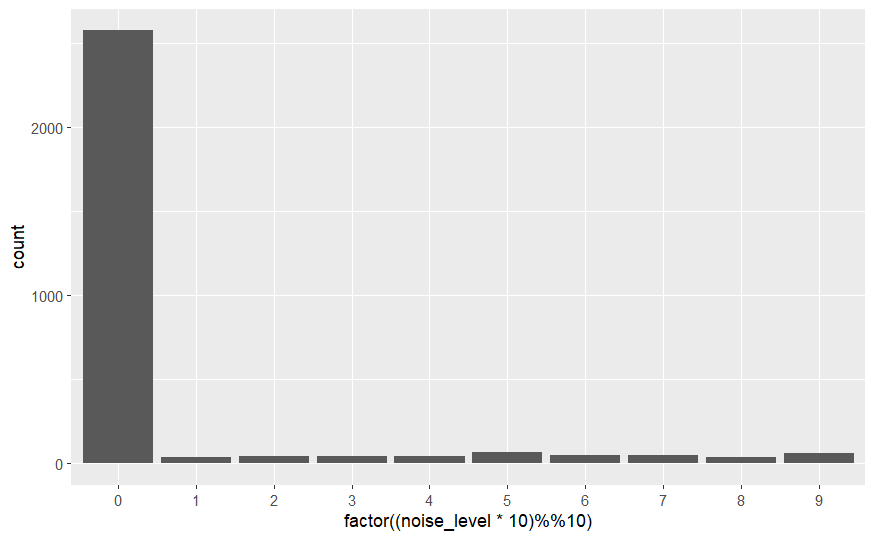
\includegraphics[width=0.8\textwidth]{../plots/afronding noise.png}
        \caption{weird rounding noise}
        \label{fig:rounding}
\end{figure}


\begin{figure}[h!]
        \centering
        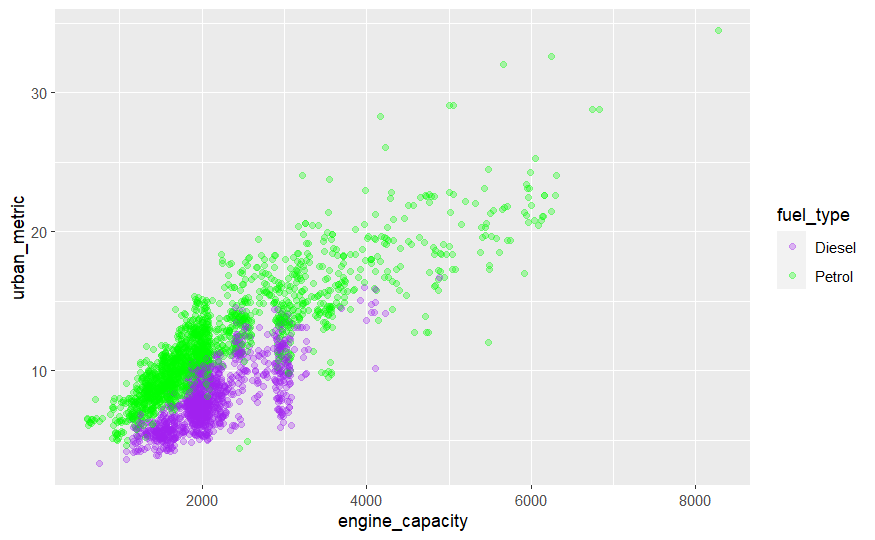
\includegraphics[width=0.8\textwidth]{../plots/plt1.png}
        \caption{plt1}
        \label{fig:plt1}
\end{figure}


\begin{figure}[h!]
        \centering
        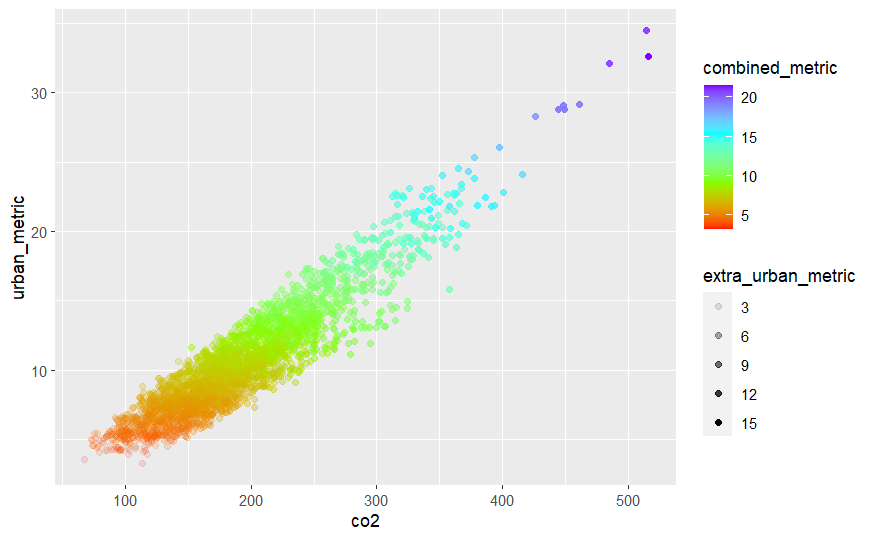
\includegraphics[width=0.8\textwidth]{../plots/plt2.png}
        \caption{plt2}
        \label{fig:plt2}
\end{figure}   

\begin{figure}[h!]
        \centering
        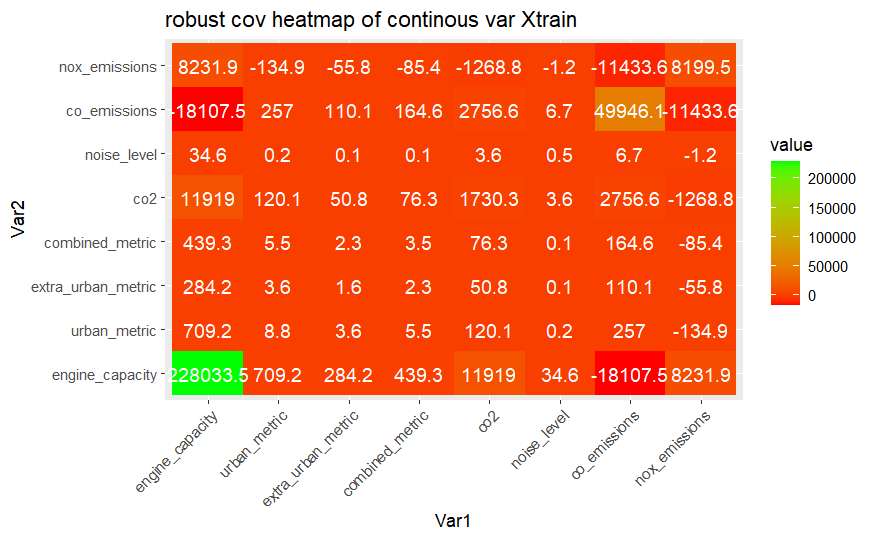
\includegraphics[width=0.8\textwidth]{../plots/rob_cov.png}
        \caption{robust covariance}
        \label{fig:robcov}
\end{figure} 

\begin{figure}[h!]
        \centering
        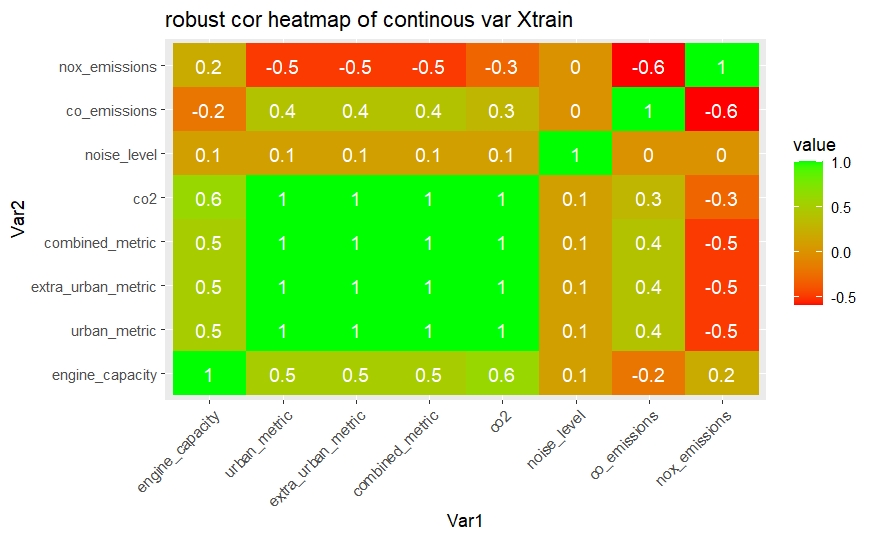
\includegraphics[width=0.8\textwidth]{../plots/rob_cor.png}
        \caption{robust correlation}
        \label{fig:robcor}
\end{figure}


\begin{figure}[h!]
        \centering
        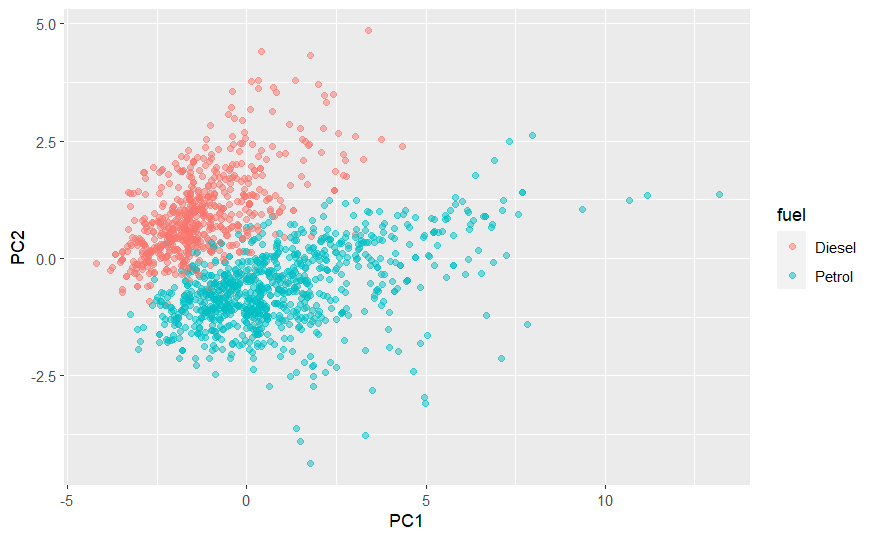
\includegraphics[width=0.8\textwidth]{../plots/pca.png}
        \caption{biplot}
        \label{fig:biplot}
\end{figure}

\begin{figure}[h!]
        \centering
        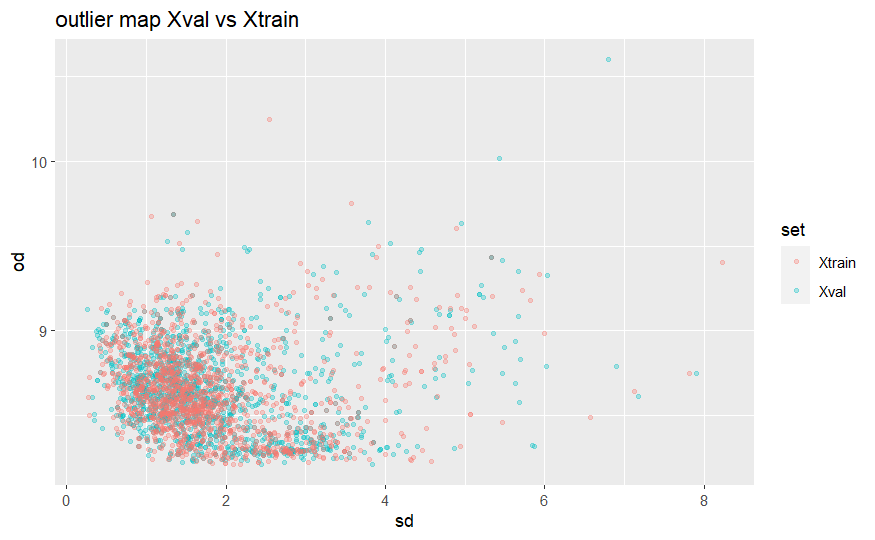
\includegraphics[width=0.8\textwidth]{../plots/val_PCA.png}
        \caption{validation pca}
        \label{fig:valpca}
\end{figure}

\begin{figure}[h!]
        \centering
        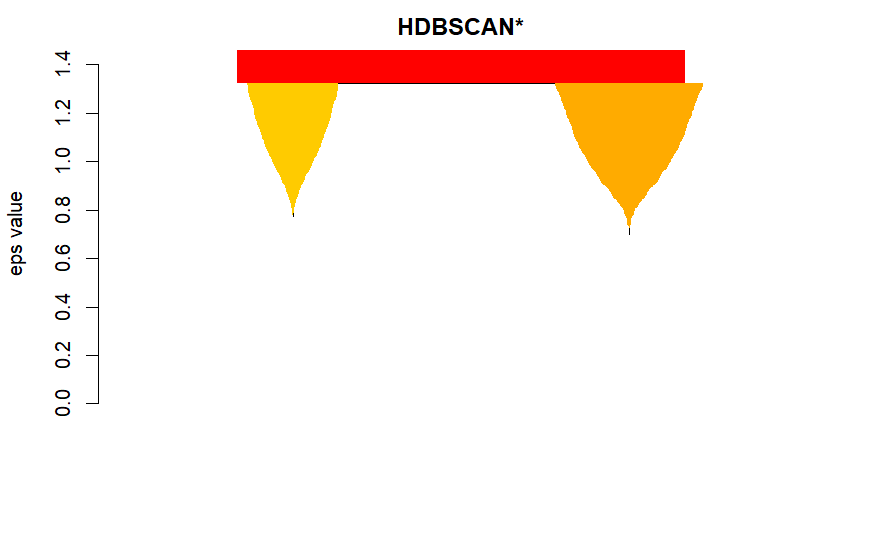
\includegraphics[width=0.8\textwidth]{../plots/hdbs1.png}
        \caption{hdbs1}
        \label{fig:hdbs1}
\end{figure}

\begin{figure}[h!]
        \centering
        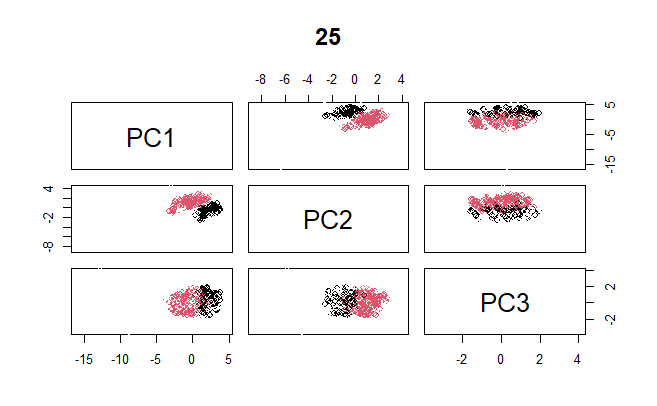
\includegraphics[width=0.8\textwidth]{../plots/hdbs2.png}
        \caption{hdbs2}
        \label{fig:hdbs2}
\end{figure}

\begin{figure}[h!]
        \centering
        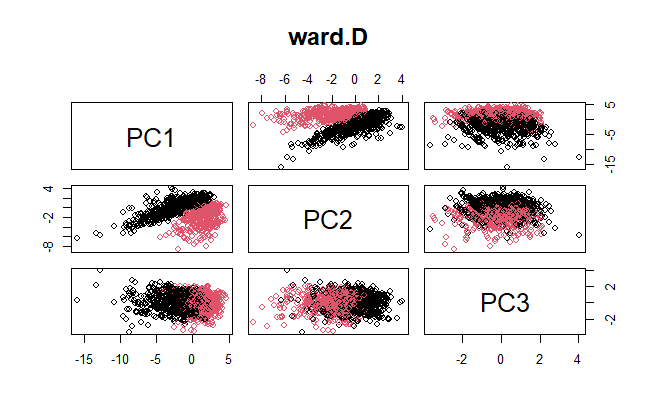
\includegraphics[width=0.8\textwidth]{../plots/ward.png}
        \caption{ward}
        \label{fig:ward}
\end{figure}    

\begin{figure}[h!]
        \centering
        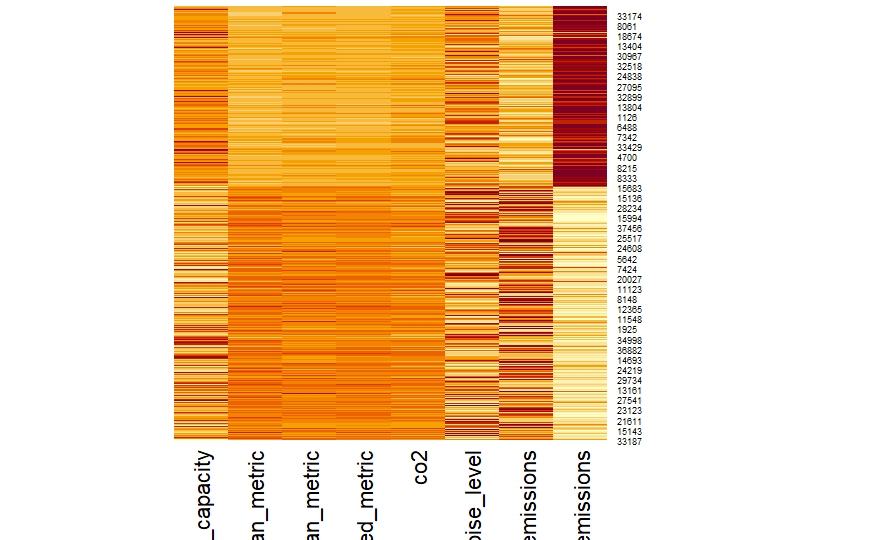
\includegraphics[width=0.8\textwidth]{../plots/heatmap.png}
        \caption{heatmap}
        \label{fig:heatmap}
\end{figure}

\begin{figure}[h!]
        \centering
        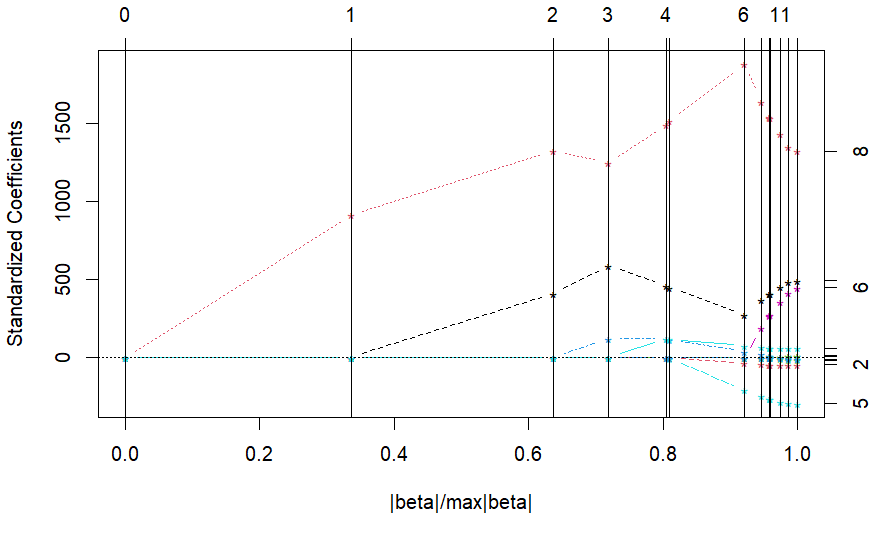
\includegraphics[width=0.8\textwidth]{../plots/lars1.png}
        \caption{lars1}
        \label{fig:lars1}
\end{figure}

\begin{figure}[h!]
        \centering
        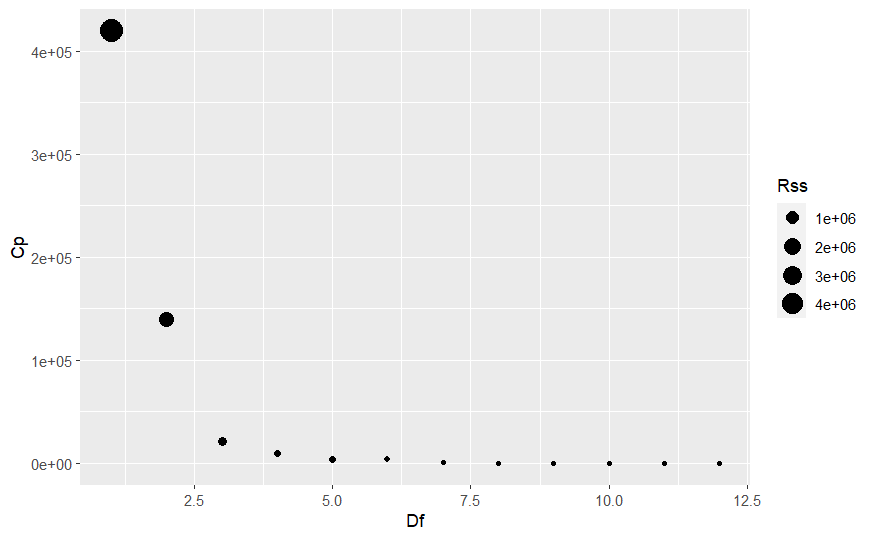
\includegraphics[width=0.8\textwidth]{../plots/lars2.png}
        \caption{lars2}
        \label{fig:lars2}
\end{figure}

\begin{figure}[h!]
        \centering
        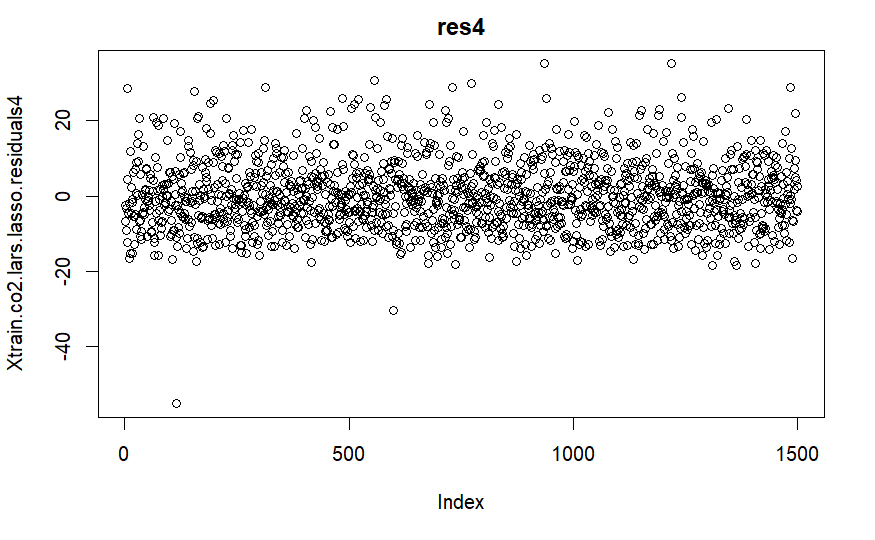
\includegraphics[width=0.8\textwidth]{../plots/lars3.png}
        \caption{lars3}
        \label{fig:lars3}
\end{figure}

\begin{figure}[h!]
        \centering
        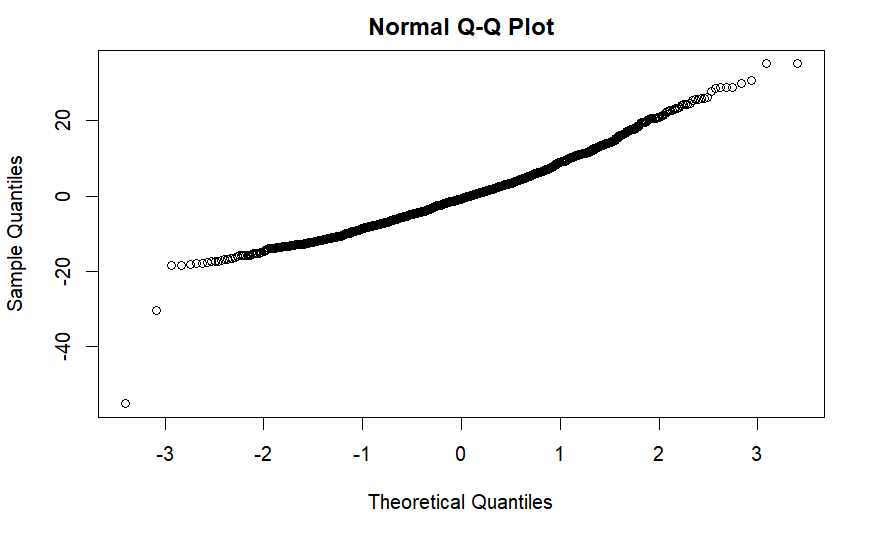
\includegraphics[width=0.8\textwidth]{../plots/lars4.png}
        \caption{lars4}
        \label{fig:lars4}
\end{figure}

\begin{figure}[h!]
        \centering
        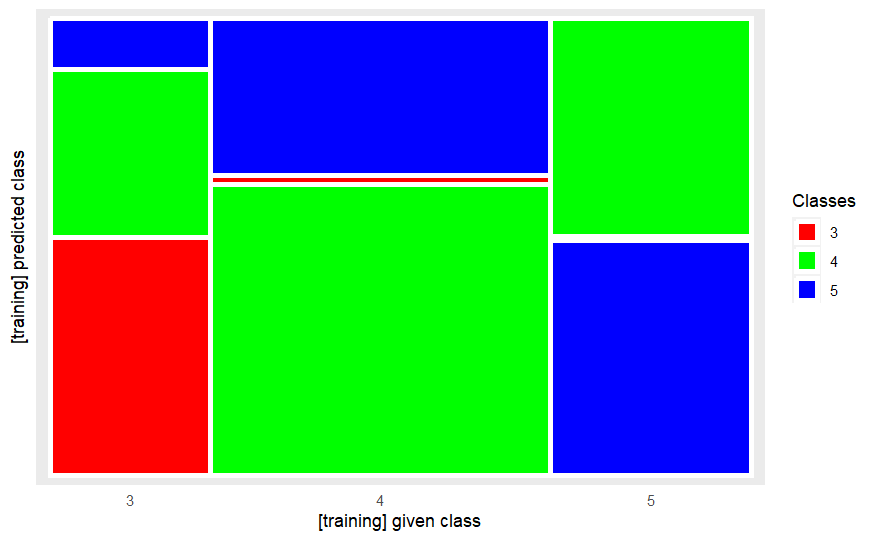
\includegraphics[width=0.8\textwidth]{../plots/mos_knn_train.png}
        \caption{knn train}
        \label{fig:knntrain}
\end{figure}

\begin{figure}[h!]
        \centering
        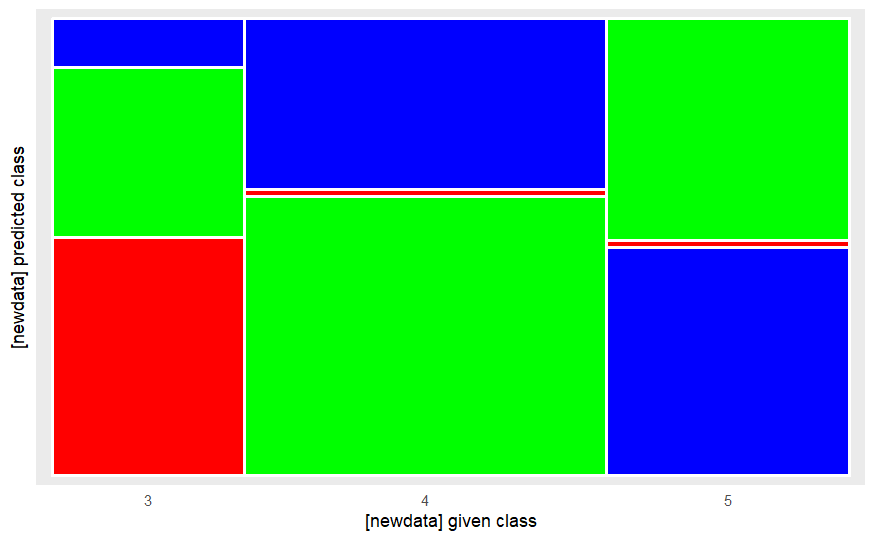
\includegraphics[width=0.8\textwidth]{../plots/mos_knn_val.png}
        \caption{knn validation}
        \label{fig:knnval}
\end{figure}
\end{document}